\chapter{基督擊敗撒但（20:1-20:15）}

第二十章最後把我們帶到白色大寶座前。到了那一天，所有人都要站在神面前。無論大小，無論在世上擁有多少權力、財富或名望，都不能逃避最後的審判。死亡和陰間也不能成為永遠的避難所。生命冊展開，人的一生都要在神面前顯明。

此章也有不同的解釋角度。那一千年究竟是字面上的一千年，還是象徵一段完整的時期？「第一次復活」是指身體的復活，還是指屬靈的生命？基督是在地上作王一千年，還是祂如今已經在掌權？撒但被捆綁又是什麼意思？因爲歷代對這些問題認真思考過，就形成了不同的末世論立場。

然而，當我們閱讀這一章時，不要讓這些問題遮住了約翰所要我們看見的中心。撒但不是最終的王，基督才是。而我們更應該自問的是：「既然基督必得勝，我今天應當怎樣忠心跟隨祂？」

\section{撒但被捆綁。基督一同作王}
\begin{figure}[htbp]
    \centering
    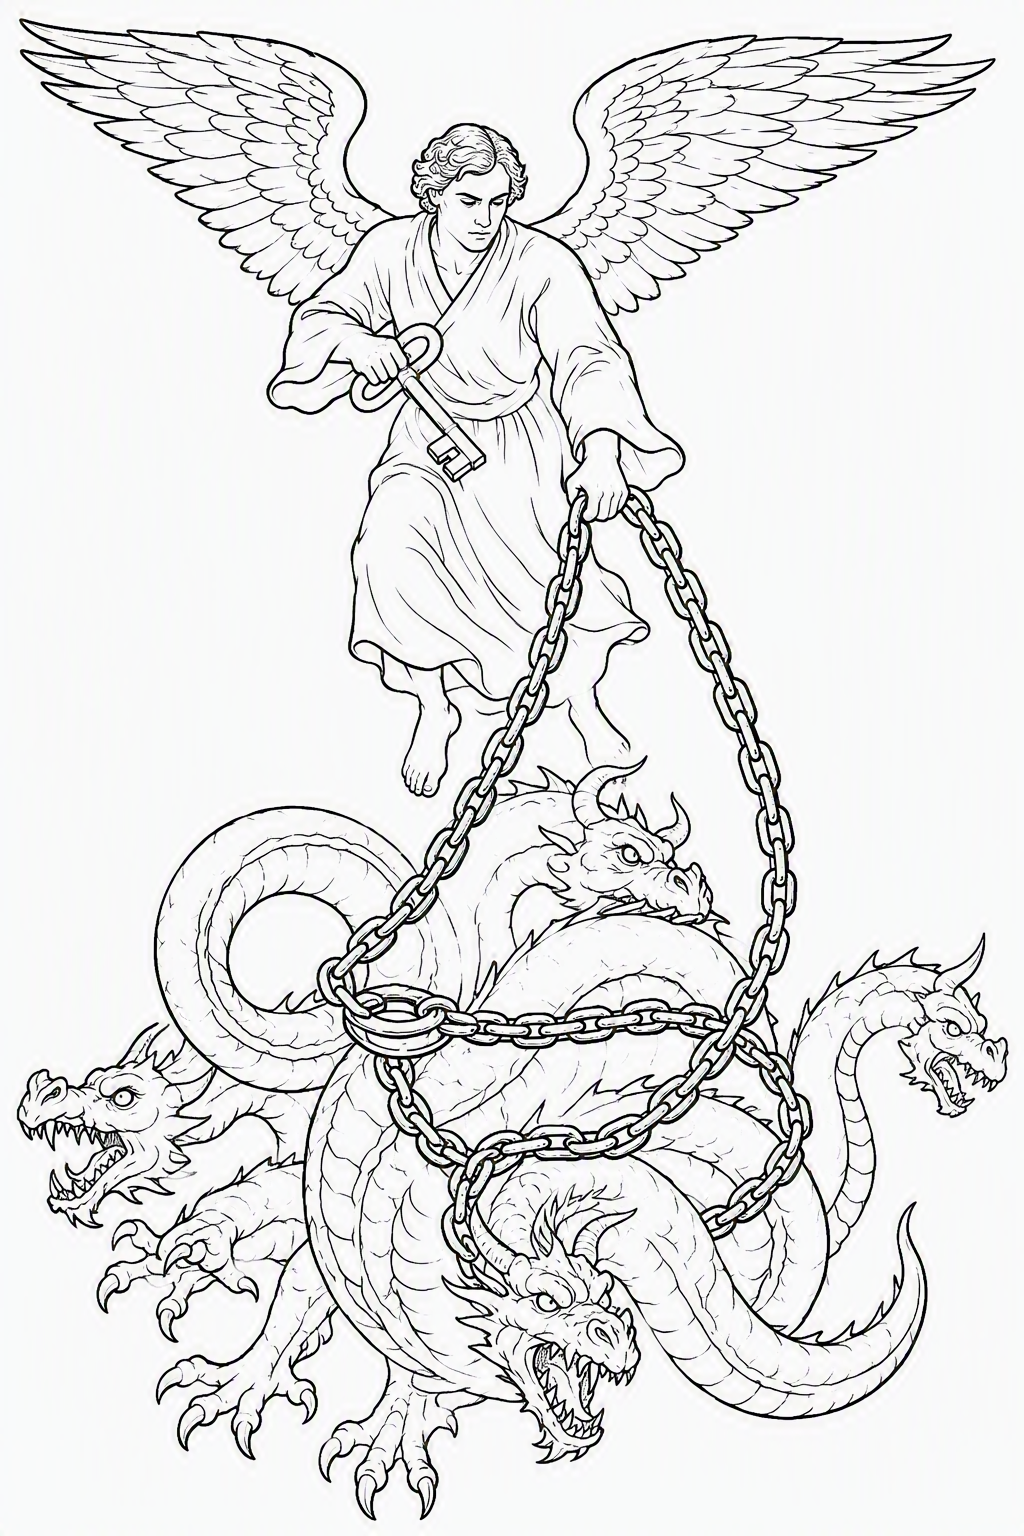
\includegraphics[
    width=0.6\textwidth, 
    trim=0 0 0 0, 
    clip]{images/rev20-satan-bound.png}
    %\caption{}
    %\label{}
\end{figure}




\begin{ScriptureBox}



\item[20:1] 我又看見一位天使從天降下、手裡拿著無底坑的鑰匙、和一條大鍊子。

\item[20:2] 他捉住那龍、就是古蛇、又叫魔鬼、也叫撒但、把他捆綁一千年、

\item[20:3] 扔在無底坑裡、將無底坑關閉、用印封上、使他不得再迷惑列國、等到那一千年完了．以後必須暫時釋放他。

\item[20:4] 我又看見幾個寶座、也有坐在上面的、並有審判的權柄賜給他們．我又看見那些因為給耶穌作見證、並為　神之道被斬者的靈魂、和那沒有拜過獸與獸像、也沒有在額上和手上受過他印記之人的靈魂．他們都復活了、與基督一同作王一千年。

\item[20:5] 這是頭一次的復活。其餘的死人還沒有復活、直等那一千年完了。

\item[20:6] 在頭一次復活有分的、有福了、聖潔了．第二次的死在他們身上沒有權柄．他們必作　神和基督的祭司、並要與基督一同作王一千年。

\item[20:7] 那一千年完了、撒但必從監牢裡被釋放、

\end{ScriptureBox}

讀了以上的經文，我們知道撒但雖然仍然存在，卻被神綑綁，不能迷惑列國。那些忠心跟隨基督的人，會與基督一同作王。

然而你可能就問，為什麼不是「立刻」消滅撒但，而是先捆綁？%
這個問題不是小問題，歷史上從教父時代到如今，就已經多所討論。所以我們也花一點時間了解一下。

\subsection{為什麼不是「立刻」消滅撒但？}

早期教父如游斯丁（Justin Martyr）和愛任紐（Irenaeus），大多理解「捆綁」是將來某一天會發生，基督在大患難之後再度降臨，捆綁撒但，並在地上作王一千年。這可稱為「前千禧年」的解釋。「前」，是基督再臨在千禧年之前。

到了奧古斯丁（Augustine），解釋出現重要轉變。他在《上帝之城》中敘述，撒但已經被捆綁。這「一千年」是「從基督降臨直到末日的教會時代。」這種捆綁並不是說撒但完全不能活動，而是神限制牠「迷惑列國」的能力，使福音得以向列國傳開。中世紀西方教會大體延續奧古斯丁的理解，將「一千年」視為教會時代；撒但仍然可以試探、攻擊人，但牠的權勢受到神的限制，直到末日才接受最終審判。這可稱為「無千禧年」的解釋。

到了近代，前千禧年派受到許多的重視。


\subsection{誰是地上的居民？}

既然復活的聖徒與基督一同作王管理，你可能會問誰是地上的居民？千禧年中可以區分為兩類人：
\begin{itemize}
\item 復活的聖徒：有榮耀、不朽壞的身體。與基督一同作王。
\item 肉身居民：仍然是必死的身體。活在基督的統治之下，並生養後代。
\end{itemize}


\subsection{千禧年}

對這一千年的解釋，可以有前千禧年派，後千禧年派，和無千禧年派等觀點。我特別製表於「附錄：千禧年觀」。我在這裡先列出前千禧年派的解釋。前千禧年派認為，基督會在千禧年之前親自再來，捆綁撒但，使殉道的聖徒復活，並在地上與他們一同作王一千年，之後撒但被釋放、發動最後的叛亂，隨即被永遠扔在火湖裡。

無論是前千禧年派，後千禧年派，或是無千禧年，啟示錄二十章最終都指向同一個高潮：撒但被擊敗，基督的國度進入終極的榮耀。

\section{最後的戰役：歌革與瑪各（Gog Magog）}

\begin{figure}[htbp]
    \centering
    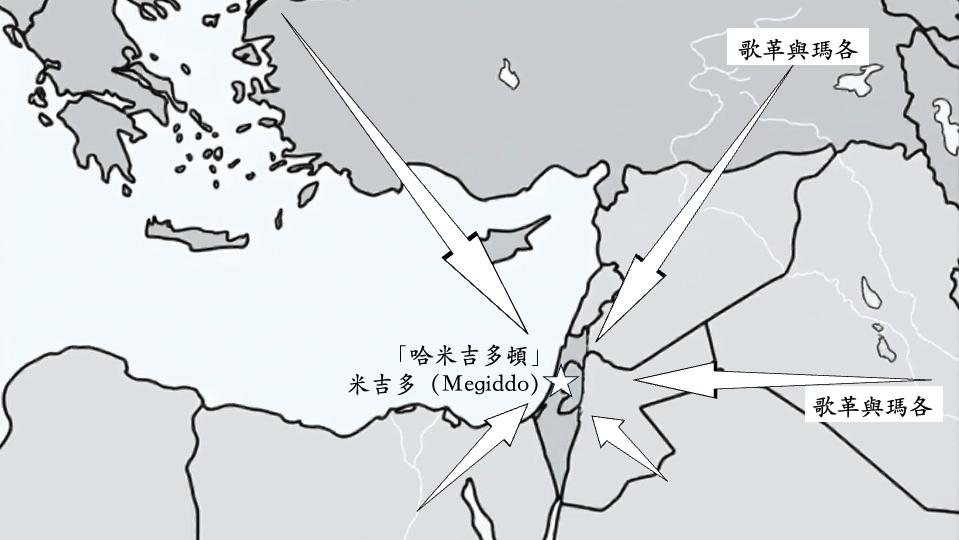
\includegraphics[
    width=1\textwidth, 
    trim=0 0 0 0, 
    clip]{images/armageddon.png}
    %\caption{}
    %\label{}
\end{figure}



\begin{ScriptureBox}

\item[20:8] 出來要迷惑地上四方的列國、〔方原文作角〕就是歌革和瑪各、叫他們聚集爭戰．他們的人數多如海沙。

\item[20:9] 他們上來遍滿了全地、圍住聖徒的營、與蒙愛的城．就有火從天降下、燒滅了他們。

\item[20:10] 那迷惑他們的魔鬼、被扔在硫磺的火湖裡、就是獸和假先知所在的地方．他們必晝夜受痛苦、直到永永遠遠。

\end{ScriptureBox}




歌革與瑪各雖然只在啟示錄20章出現一節經文，但這兩個名稱早已出現在以西結書38至39章。以西結所描述的歌革，是從「北方極處」而來，率領眾多列國攻擊神的子民；到了啟示錄，歌革與瑪各則被描述為從「地的四方」聚集而來，圍住「蒙愛的城」。然而，當敵軍聚集之後，「就有火從天降下來，燒滅了他們」（啟示錄20:9）。

啟示錄在這裡採用了稍微不同的視角，來描述以西結書已經描述的這場末世戰役。
這是神學上的「末世論的重構」（Eschatological reconfiguration）：啟示錄不是單純重複舊約的末世預言，而是將舊約既有的末世意象重新組合、重新定位，使它們在基督的救贖與末世審判的框架中產生新的功能。

值得注意的是，在啟示錄19章，基督已經擊潰在哈米吉多頓集結的敵對勢力，此處20章的歌革與瑪各，則從另一個角度再次描寫此
邪惡勢力的覆滅。
哈米吉多頓與歌革、瑪各都顯示著，邪惡雖然可以在歷史中最後一次聚集，牠的結局已定。

\section{最後的審判：白色大寶座前的終極審判}

\begin{ScriptureBox}

\item[20:11] 我又看見一個白色的大寶座、與坐在上面的．從他面前天地都逃避、再無可見之處了。

\item[20:12] 我又看見死了的人、無論大小、都站在寶座前．案卷展開了．並且另有一卷展開、就是生命冊．死了的人都憑著這些案卷所記載的、照他們所行的受審判。

\item[20:13] 於是海交出其中的死人．死亡和陰間也交出其中的死人．他們都照各人所行的受審判。

\item[20:14] 死亡和陰間也被扔在火湖裡．這火湖就是第二次的死。

\item[20:15] 若有人名字沒記在生命冊上、他就被扔在火湖裡。

\end{ScriptureBox}

約翰看見一個「白色的大寶座」，在祂面前，天地都逃避，再無可見之處。現今的天地將要過去，神的終極審判已經來到。死了的人，無論大小，都站在寶座前，案卷展開，另有一卷就是生命冊。眾人都要按照案卷所記載的，照各人所行的受審判。沒有人能逃避這最後的審判。每一個人都要站在神的審判台前，而最後的結局只有生命與第二次的死兩種。

\begin{figure}[htbp]
    \centering
    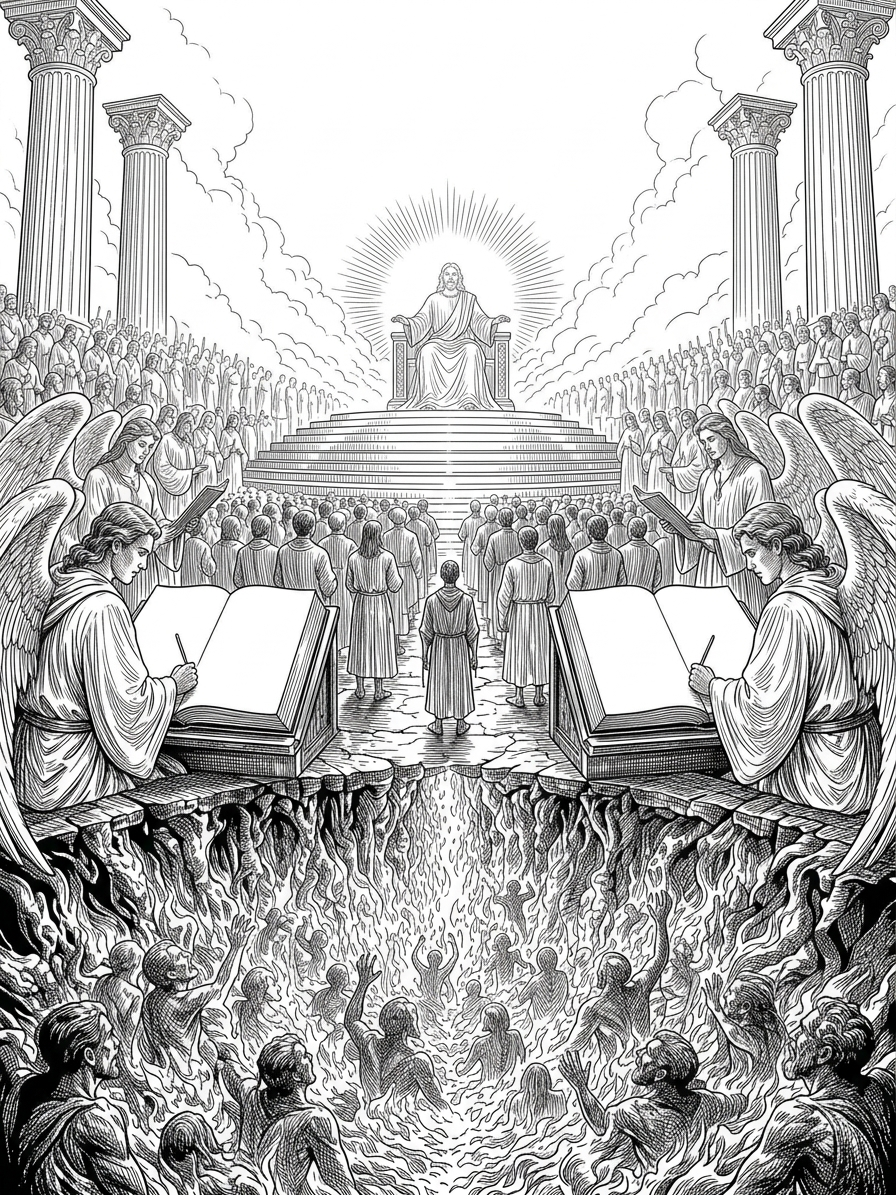
\includegraphics[
    width=1\textwidth, 
    trim=0 0 0 0, 
    clip]{images/white_throne_judgement.jpg}
    %\caption{}
    %\label{}
\end{figure}

\section*{小組討論題}

\begin{enumerate}
    
    \item 讀20:11-15的白色大寶座。這段經文帶給你最大的感受是警醒、敬畏、安慰，還是盼望？為什麼？

    \item 如果你確信基督最終必得勝、撒但必被擊敗、死亡必被除去，你今天的生活會有什麼不同？在家庭、工作、教會或苦難中，你最需要持守的是什麼？
\end{enumerate}
